\typeout{Informe Proyecto 01 - Reductor SAT X-SAT}

\documentclass{article}
\usepackage{acra}
\usepackage[utf8]{inputenc}
\usepackage{hyperref}
\usepackage{graphicx}
\usepackage[spanish]{babel}
\usepackage{listings}
\usepackage{xcolor}

\definecolor{codegreen}{rgb}{0,0.6,0}
\definecolor{codegray}{rgb}{0.5,0.5,0.5}
\definecolor{codepurple}{rgb}{0.53,0.1,0.6}
\definecolor{codeblue}{rgb}{0.53,0.6,0.8}
\definecolor{backcolour}{rgb}{0.95,0.95,0.95}
\lstdefinestyle{mystyle}{
    backgroundcolor=\color{backcolour},
    commentstyle=\color{codegreen},
    keywordstyle=\color{codeblue},
    numberstyle=\tiny\color{codegray},
    stringstyle=\color{codepurple},
    basicstyle=\ttfamily\footnotesize,
    breakatwhitespace=false,
    breaklines=true,
    captionpos=b,
    keepspaces=true,
    numbers=left,
    numbersep=5pt,
    showspaces=false,
    showstringspaces=false,
    showtabs=false,
    tabsize=2
}

\lstset{style=mystyle}


\title{Informe de Taller - Regresión lineal}
\author{Afanador, S. \\ Universidad del Valle \\ Probabilidad y estadística \\ \it{02 Marzo 2022}}


\begin{document}

\maketitle
\selectlanguage{spanish}
\begin{abstract}
Este informe busca proponer un modelo sencillo de regresión lineal para hallar la relación entre el cilindraje medido en centímetros cúbicos (CC) de los motores de un dataset de autos con su respectiva potencia medida en caballos de fuerza(HP).
\end{abstract}

\section{Descripción de conjunto de datos}
Este conjunto de datos tiene las siguientes las columnas referentes al nombre del auto \textit{name}, el año del modelo del vehículo \textit{year}, el precio de venta del vehículo en USD \textit{selling\_price}, La cantidad de kilómetros recorridos por el vehículo \textit{km\_driven}, el tipo de vendedor \textit{seller\_type}, el tipo de transmisión de vehículo \textit{transmission}, el orden del propietario final del vehículo \textit{owner}, el kilometraje en Km \textit{mileage}, el tamaño del motor en centimetros cúbicos \textit{engine}, la potencia máxima del motor en HP \textit{max\_power}, el torque del motor Nm \textit{torque}, y la cantidad de asientos que tiene el auto \textit{seats}.\par

Este conjunto de datos cuenta con 8128 registros, fue obtenido del sitio web de Kaggle\footnote{Dataset: \url{https://www.kaggle.com/nehalbirla/vehicle-dataset-from-cardekho}} de donde especificamente se usó el archivo \textit{Car details v3.csv}.

\section{Limpieza de datos}
Se inicia limpiando los datos de inconsistencias y anormalidades, como primero paso se eliminan todos las filas que tengan algún dato faltante en al menos una de sus columnas. Seguidamente se elimina el texto de los valores numéricos, como es el caso de la columna \textit{max\_power} que tiene siempre las unidades \textit{bhp} y el caso de la columna \textit{engine} que para todos sus valores tiene las unidades \textit{CC}.\par
Después eliminan las columnas que no se usarán o que tienen datos de tipo \textit{String} como es el caso de \textit{name}, \textit{seller\_type}, \textit{transmission}, \textit{owner}, \textit{torque}.

\section{Criterio para elección de las variables}
Una vez que los datos están limpios de anormalidades y se tienen las variables justas con cantidades numéricas se procede a crear una matriz de correlación para conocer cuales de las variables tienen mejor relación entre si.\par

Se obtienen los siguientes resultados usando la librería \textit{corrplot} donde se puede evidenciar uno de los pares de variables que mejor correlación tienen son \textit{engine} y la variable \textit{max\_power} con un valor de \(0.743\) relacionando de manera directa el tamaño del motor con la potencia máxima que puede producir.\par

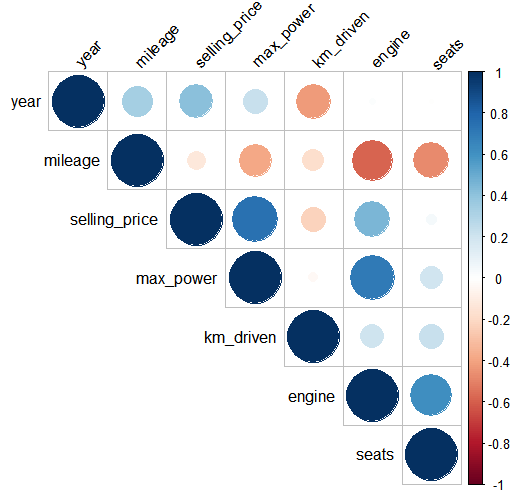
\includegraphics[scale=0.55, trim={0cm 0cm 0cm 0cm}, clip]{graphs/conclusion1.png}

\section{Creación del modelo}
Después de escoger las variables \textit{engine} y \textit{max\_power} como las candidatas para ser analizadas se procede a visualizar gráficamente los datos de ambas variables para evidenciar el comportamiento que tienen entre sí.
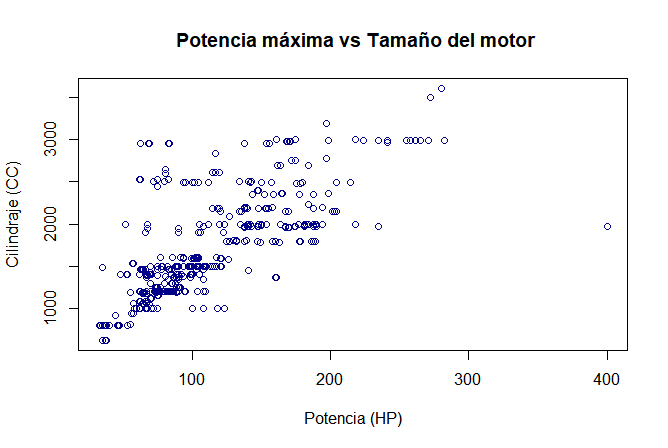
\includegraphics[scale=0.45, trim={0cm 0cm 0cm 0cm}, clip]{graphs/conclusion2.png}

\section{Parámetros del modelo de regresión}
Para crear el modelo se uso la función \textit{lm} del paquete estandar de R para hallar los valores de intercepto \(\beta_0\) y pendiente de la función lineal \(\beta_1\) que representa el modelo que mas se ajusta al valor esperado del Cilindraje de un motor de auto dada su potencia en caballos de fuerza.

\[y = 549.8 + 9.92x\]

Teniendo en cuenta los valores anteriores, la gráfica del modelo junto con los datos quedaría de la siguiente asi:

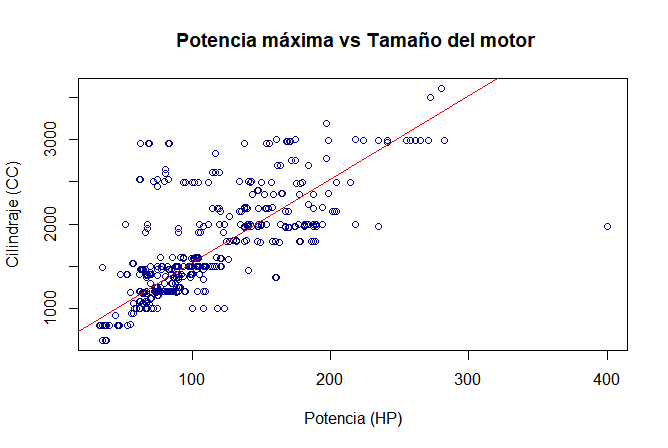
\includegraphics[scale=0.45, trim={0cm 0cm 0cm 0cm}, clip]{graphs/conclusion3.png}

\section{Código fuente}
 Acontinuación el código usado para calcular los valores del modelo simple de regresión y la creación de los gráficos incluidos en el informe.
\lstinputlisting[language=R]{script.R}

\section{Agradecimientos}
Al profesor Wilmar Sepulveda Herrera porque sin su ayuda, paciencia y conocimiento no habría sido posible este trabajo.

\end{document}